\documentclass{rapport_stage}

% package ajouté au dessus de la template

\usepackage{xcolor}
\usepackage{csquotes}
\usepackage{bookmark}
\usepackage{enumitem}
\usepackage{pifont}
\usepackage[style=ieee,backref=true]{biblatex}

% Lien vers la bibliographie

\bibliography{bibliography_rapport_de_stage}

% Variable utilisé par la template

\def\reportTitle{Analyse et Conception d'Eledone : un outil de déploiement de simulations pour l'utilisateur profane} % Titre du rapport de stage

\def\reportAuthor{Théo Piacentini}
\def\reportAuthorEmail{\email{theo.piacentini@gmail.com}} % Courriel de l'élève

\def\reportSupervisor{Jean-François Santucci, Laurent Capocci} % Nom des tuteurs

\def\reportCompany{UMR 6134 CNRS} % Nom de l'entreprise d'accueil

% % ====================== Début Document  ==========================



\begin{document}

\maketitle
\pagenumbering{roman}

\cleardoublepage

Théo Piacentini \\
Résidence Le Boticelli \\
20620 Biguglia \\
+33 (0)7 77 78 55 54 \\
\href{mailto:theo.piacentini@gmail.com}{\nolinkurl{theo.piacentini@gmail.com}}

\smallskip

Jean-François Santucci \\
Professeur Titulaire \\
Université de Corse "Pasquale Paoli"\\
UMR CNRS 6134\\
Quartier Grossetti\\
BP 52, 20250 Corte\\
tel : +33 4 95 45 02 30\\
\href{mailto:santucci-j@univ-corse.fr}{\nolinkurl{santucci-j@univ-corse.fr}}

\smallskip

Laurent Capocci \\
Maitre de Conférence en Informatique \\
Université de Corse "Pasquale Paoli"\\
UMR CNRS 6134\\
Quartier Grossetti\\
BP 52, 20250 Corte\\
tel : +33 4 95 45 02 30\\
\href{mailto:capocchi@univ-corse.fr}{\nolinkurl{capocchi@univ-corse.fr}}

\cleardoublepage
\phantomsection
\section*{Remerciements}
\addcontentsline{toc}{chapter}{Remerciements}

{\color{green}
  à compléter
}

\clearpage

\renewcommand{\baselinestretch}{0.5}\normalsize
\tableofcontents
\renewcommand{\baselinestretch}{1.0}\normalsize
\cleardoublepage

\pagenumbering{arabic}
\setcounter{page}{1}

\chapter*{Introduction}  % no number
\addcontentsline{toc}{chapter}{Introduction} % add it to the ToC

\section*{Pourquoi choisir ce stage ?}

\begin{itemize}[label=$\bullet$]
  \item J'ai toujours été intéressé par la recherche je voulais donc découvrir le metier
  \item Je voulais découvrir la simulation l'un des seuls grands domaine de l'Informatique que je n'ai pas encore étudié
  \item L'approche scientifique de l'Informatique et le formalisme sont des sujets qui me tiennent à cœur
  \item visé une thèse est un objectifs je dois donc passer par des stages dans la recherche
\end{itemize}

\section*{Quels enjeux ?}

\begin{itemize}[label=$\bullet$]
  \item Le but pour moi est d'avoir une première experience dans la rechercher et dans l'informatique professionnel
  \item L'idée est de trouver des sujet à approfondir pour l'année prochaine
\end{itemize}

\cleardoublepage

% ====================== PARTIE 1  ==========================




\part{Présentation du stage}

\chapter{Présentation de l'Organisme}

\begin{itemize}[label=$\bullet$]
  \item Présenter l'UMR \cite{santoni_presentation_2022}
  \item voire site web
\end{itemize}

\section*{Laboratoire Sciences Pour l'Environnement de l'Université de Corse}

\begin{itemize}[label=$\bullet$]
  \item présenter rapidement le laboratoire dans son ensemble
\end{itemize}

\section*{Le Projet SISU : Simulation Informatique et Systèmes Ubiquitaires}

\begin{itemize}[label=$\bullet$]
  \item Expliquer le projet SISU
  \item Trouver les différents sujet lié a SISU
\end{itemize}

\cleardoublepage

\chapter{Présentation de la tâche effectuée}

\section*{Semaine 1}

\begin{itemize}[label=$\bullet$]
  \item choix du projet rdv à l’IUT de Corte
  \item création de maquettes
  \item création de schemas
  \item Lecture des papiers
  \item début de l'état de l'art
\end{itemize}

\section*{Semaine 2}

\begin{itemize}[label=$\bullet$]
  \item visioconférence pour discute de l'avancé du projet et des décisions lié à celui-ci
  \item Découverte et utilisation de LaTeX pour l'écriture du rapport
  \item création du plan du rapport / projet
  \item avancé état de l'art
  \item Création de schemas
  \item Recherche de ressources lié à la simulation et aux systèmes distribués
  \item liaison des outils de schemas et de ressources avec LaTeX
\end{itemize}

\section*{Semaine 3}

\begin{itemize}[label=$\bullet$]
  \item The first item of the list.
\end{itemize}

\section*{Semaine 4}

\begin{itemize}[label=$\bullet$]
  \item The first item of the list.
\end{itemize}

\chapter{Définition du projet et de ses objectifs}

\section{Les origines scientifiques}

\begin{itemize}[label=$\bullet$]
  \item décrire les papiers de M. Santucci et M.Capocchi \cite{capocchi_devs_2022} \cite{capocchi_towards_2023}
  \item description succinct de DEVS
\end{itemize}

\section{Description du projet}

\begin{itemize}[label=$\bullet$]
  \item Le concept est de créer un CMS autour de la simulation
  \item au vue de la durée de stage un se contentera de la phase d'analyse et du conception du projet
  \item Le projet doit être une base la plus solide possible que se soit du côte des sources scientifiques que dans la conception même du logiciel
\end{itemize}

\section{Les objectifs}

\begin{itemize}[label=$\bullet$]
  \item The first item of the list.
\end{itemize}

\section{Explication de notre approche}

\begin{itemize}[label=$\bullet$]
  \item au vue des objectifs on va considérer que tout choix technologique rationnelle est faisable
  \item On va tout découpler au maximum pour rendre le travail en équipe possible
\end{itemize}

% ====================== PARTIE 2  ==========================



\part{Analyse}

\begin{itemize}[label=$\bullet$]
  \item The first item of the list.
\end{itemize}

\chapter{État de l'art}


test des footnotes \footnote{test}
\begin{itemize}[label=$\bullet$]
  \item Introduction de l'état de l'art (pourquoi ?, comment ?)
\end{itemize}

\section{Modélisation et Simulation}

\begin{itemize}[label=$\bullet$]
  \item aaaaa
\end{itemize}

\subsection*{Définition du domaine}

\begin{itemize}[label=$\bullet$]
  \item The first item of the list.
\end{itemize}

\newpage

\subsection*{Histoire du domaine}

\begin{itemize}[label=$\bullet$]
  \item The first item of the list.
\end{itemize}

\newglossaryentry{devsg}{name={DEVS},
  description={An Application Programming Interface (API) is a particular set
      of rules and specifications that a software program can follow to access and
      make use of the services and resources provided by another particular software
      program that implements that API}}

%%% define the acronym and use the see= option
\newglossaryentry{devs}{type=\acronymtype, name={DEVS}, description={Application
      Programming Interface}, first={DEVS (Discrete Event System Specification)\glsadd{devsg}}, see=[Glossary:]{devsg}}

\subsection*{\gls{devs}: Une approche formelle de la Simulation }

\begin{itemize}[label=$\bullet$]
  \item The first item of the list.
\end{itemize}

\subsection*{Les autres points de vue}

\begin{itemize}[label=$\bullet$]
  \item The first item of the list.
\end{itemize}

\section{Systèmes de gestion de contenu}

\newglossaryentry{cmsg}{name={CMS},
  description={definition des CMS}}

%%% define the acronym and use the see= option
\newglossaryentry{cms}{type=\acronymtype, name={CMS}, description={Content Management System}, first={CMS (Content Management System)\glsadd{cmsg}}, see=[Glossary:]{cmsg}}

\subsection*{Définition des \gls{cms}}

\begin{itemize}[label=$\bullet$]
  \item Petite histoire des CMS
        \item] donner la proportion de site web créer à partir de CMS
\end{itemize}

\subsection*{Les outils proches de notre concept}

\begin{itemize}[label=$\bullet$]
  \item Parler des CMS qui créent des applications web
  \item Parler d'anvil
  \item Parler d'amazon honeycode.
\end{itemize}

\chapter{Analyse global}

\begin{itemize}[label=$\bullet$]
  \item The first item of the list.
\end{itemize}

\begin{figure}[ht]
  \centering
  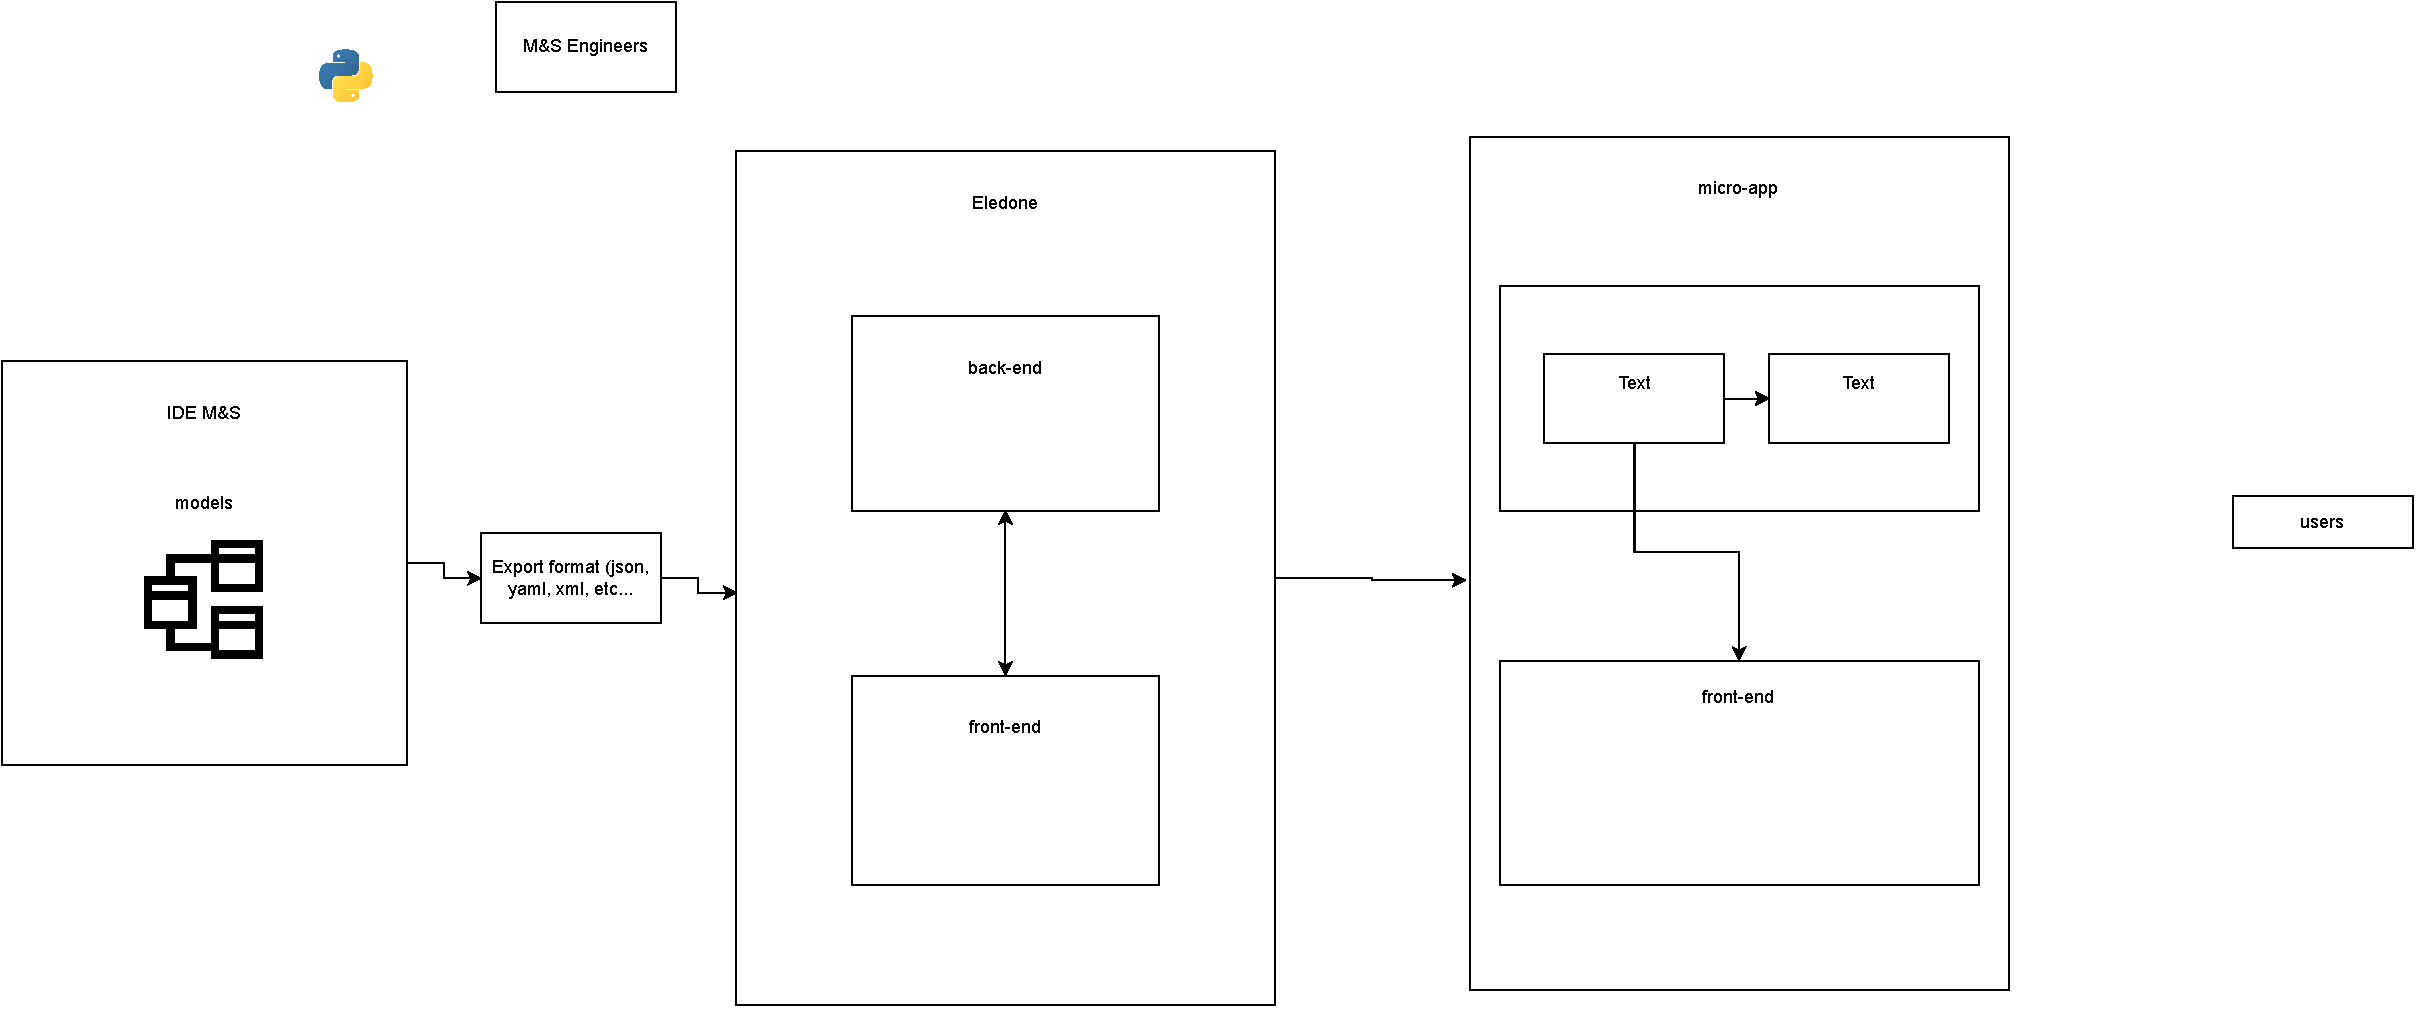
\includegraphics[width=10cm]{figures/architecture_global.pdf}
  \caption{Fonctionnement global du projet}
  \label{fig:fonctionnement-lobal-projet}
\end{figure}

\chapter{Analyse des composants individuels}

\begin{itemize}[label=$\bullet$]
  \item The first item of the list.
\end{itemize}

\section{l'export d'un modèle de simulation}

\section{l'application eledone}

\begin{figure}[ht]
  \centering
  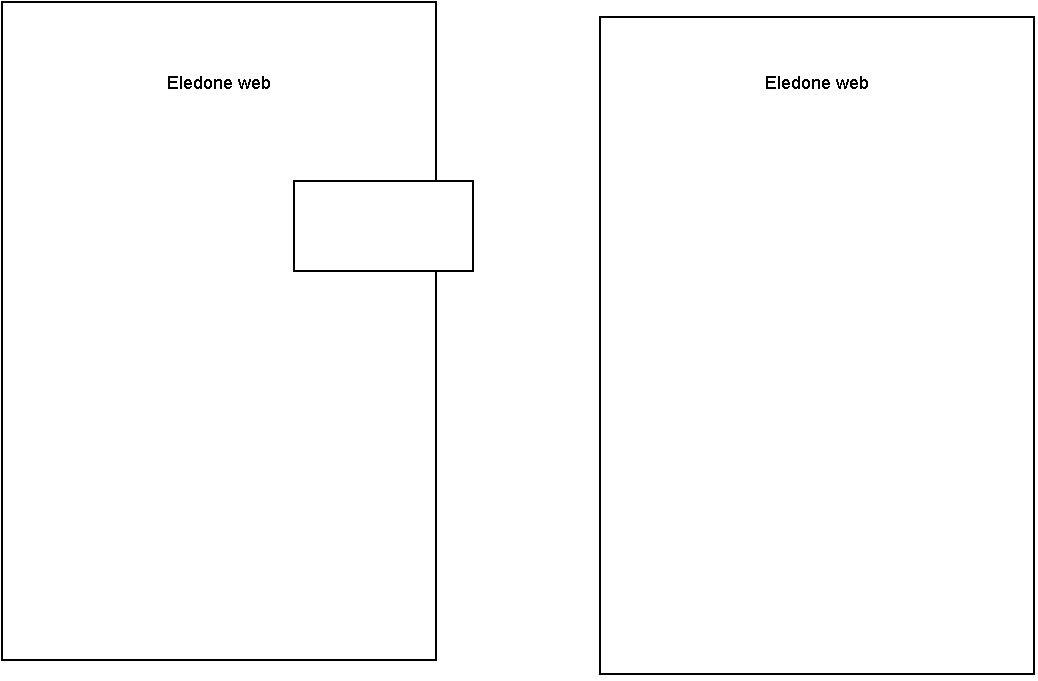
\includegraphics[width=10cm]{figures/eledone.pdf}
  \caption{schema d'analyse d'eledone}
  \label{fig:analyse-eledone}
\end{figure}

\subsection*{front-end}

\subsection*{back-end}

\section{les micro-apps générer par eledone}

\begin{figure}[ht]
  \centering
  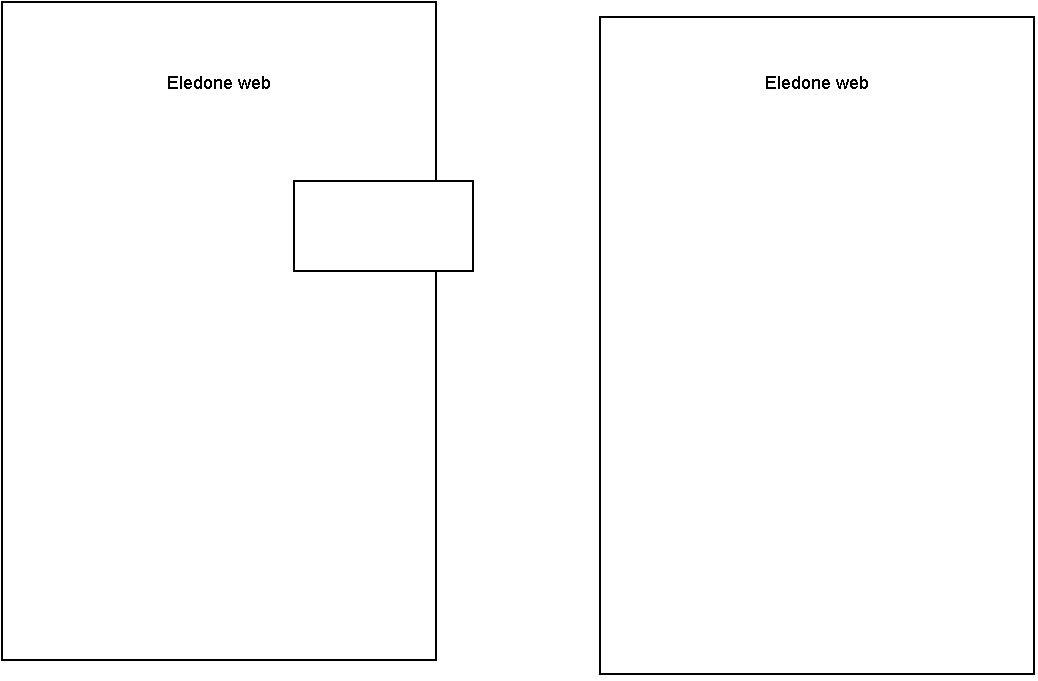
\includegraphics[width=10cm]{figures/eledone.pdf}
  \caption{schema d'analyse d'une micro-app}
  \label{fig:analyse-micro-app}
\end{figure}

\subsection*{front-end}

\subsection*{back-end}

% ====================== PARTIE 3  ==========================



\part{Conception}

\begin{itemize}[label=$\bullet$]
  \item The first item of the list.
\end{itemize}

\chapter{Conception global}

\begin{itemize}[label=$\bullet$]
  \item The first item of the list.
\end{itemize}

\chapter{Conception des composants individuels}

\begin{itemize}[label=$\bullet$]
  \item The first item of the list.
\end{itemize}

Exemple d'illustration :

\begin{figure}[ht]
  \centering
  
\includegraphics[width=10cm]{figures/univ-logo.pdf}
  \caption{Logo univ corse}
  \label{fig:logo-corse}
\end{figure}

La Figure~\ref{fig:logo-corse} représente le logo de \reportSchool{}.



\cleardoublepage

% ====================== PARTIE 4  ==========================

\part{Le projet après le stage}

\begin{itemize}[label=$\bullet$]
  \item The first item of the list.
\end{itemize}

\chapter{Pistes de réalisation}

\begin{itemize}[label=$\bullet$]
  \item The first item of the list.
\end{itemize}

\chapter{Pistes d'évaluation}

\begin{itemize}[label=$\bullet$]
  \item The first item of the list.
\end{itemize}

\chapter{Projets annexes / améliorations possibles}

\begin{itemize}[label=$\bullet$]
  \item The first item of the list.
\end{itemize}

\bookmarksetup{startatroot}

% ====================== FIN ==========================

\chapter*{Conclusion}  % no number
\addcontentsline{toc}{chapter}{Conclusion}

\begin{itemize}[label=$\bullet$]
  \item The first item of the list.
\end{itemize}% add it to the ToC


\cleardoublepage



\printbibliography[
  heading=bibintoc,
  title=Bibliographie / Webographie
]

\cleardoublepage


\listoffigures
\cleardoublepage

\listoftables
\cleardoublepage

%%% \newpage just to demonstrate that links are correct
\newpage
\printglossaries

\cleardoublepage
\renewcommand{\thesubsection}{\Roman{subsection}}



\cleardoublepage
\thispagestyle{empty}

\section*{Résumé}
\phantomsection
\addcontentsline{toc}{chapter}{Résumé}
a


  {\bf Mots-clés :}

\end{document}
